\documentclass[11pt]{article}
\usepackage[utf8]{inputenc}

%%% PAGE DIMENSIONS
\usepackage{geometry}
\geometry{a4paper}

\usepackage{graphicx}

%%% PACKAGES
\usepackage{booktabs}
\usepackage{paralist}
\usepackage{verbatim}
\usepackage{subfig}
\usepackage{chngcntr}
\usepackage{tikz}
\usepackage[colorlinks = true,
            linkcolor = black,
            urlcolor  = blue,
            citecolor = blue,
            anchorcolor = blue]{hyperref}
\usepackage[spanish]{cleveref}
\usepackage{placeins}
\usepackage{float}

%%% HEADERS & FOOTERS
\usepackage{fancyhdr}
\pagestyle{fancy}
\renewcommand{\headrulewidth}{0pt}
\lhead{}\chead{}\rhead{}
\lfoot{}\cfoot{\thepage}\rfoot{}

%%% SECTION TITLE APPEARANCE
\usepackage{sectsty}
\allsectionsfont{\sffamily\mdseries\upshape}

%%% ToC (table of contents) APPEARANCE
\usepackage[nottoc,notlof,notlot]{tocbibind} % Put the bibliography in the ToC
\usepackage[titles,subfigure]{tocloft} % Alter the style of the Table of Contents
\renewcommand{\cftsecfont}{\rmfamily\mdseries\upshape}
\renewcommand{\cftsecpagefont}{\rmfamily\mdseries\upshape} % No bold!


\graphicspath{ {images/} }

\counterwithin*{figure}{section}
\counterwithin*{figure}{subsection}
\counterwithin*{figure}{subsubsection}

\counterwithin*{table}{section}
\counterwithin*{table}{subsection}
\counterwithin*{table}{subsubsection}

\addtolength{\cftfignumwidth}{2em}

\renewcommand{\thefigure}{
  \ifnum\value{subsection}=0
    \thesection.\arabic{figure}
  \else
    \ifnum\value{subsubsection}=0
      \thesubsection.\arabic{figure}
    \else
      \thesubsubsection.\arabic{figure}
    \fi
  \fi
}

\renewcommand{\thetable}{
  \ifnum\value{subsection}=0
    \thesection.\arabic{table}
  \else
    \ifnum\value{subsubsection}=0
      \thesubsection.\arabic{table}
    \else
      \thesubsubsection.\arabic{table}
    \fi
  \fi
}

%%% END Article customizations

%%% The "real" document content comes below...

\title{\Large Seguridad en Redes\\Practica 3.2}
\author{David Antuña Rodríguez\\Javier Carrión García}
\date{}

\begin{document}
  \raggedright

  \maketitle
  \newpage

  \par
  Las MACS de las máquinas son las siguientes:
  \begin{itemize}
    \item Gateway - 08:00:27:66:bf:ba
    \item Atacante - 08:00:27:7e:9a:1a
    \item Víctima - 08:00:27:bb:76:6b
    \item Externa - 08:00:27:ec:95:27
  \end{itemize}

  \section{ARP Spoofing}
    \subsection{Ataque 1}
      \par
      El atacante ha modificado la tabla arp de la víctima para que todo el
      tráfico que esta genere pase por él. El ping no funciona porque el atacante
      actua de router pero no tiene activada la retransmisión.

      \begin{figure}[H]
        \centering
        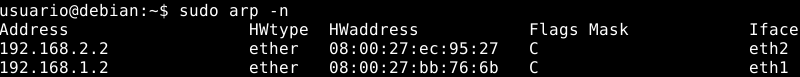
\includegraphics[width = \textwidth]{arptable_gw}
        \caption{Tabla ARP del router.}
      \end{figure}

      \begin{figure}[H]
        \centering
        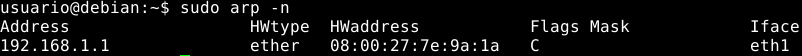
\includegraphics[width = \textwidth]{arptable_vic}
        \caption{Tabla ARP de la víctima.}
      \end{figure}
    \subsection{Ataque 2}
      \par
      El ping sí funciona porque ahora el atacante redirige el tráfico que
      intercepta, en el wireshark del atacante solo aparecen los echo request
      porque el ataque es sobre la tabla arp de la víctima y por tanto solo esta
      manda tráfico al atacante.

      \begin{figure}[H]
        \centering
        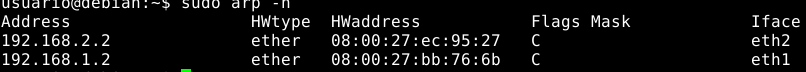
\includegraphics[width = \textwidth]{arptable_gw2}
        \caption{Tabla ARP del router.}
      \end{figure}

      \begin{figure}[H]
        \centering
        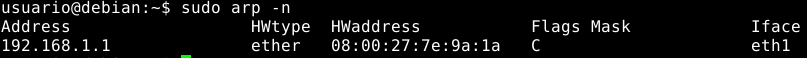
\includegraphics[width = \textwidth]{arptable_vic2}
        \caption{Tabla ARP de la víctima.}
      \end{figure}

      \begin{figure}[H]
        \centering
        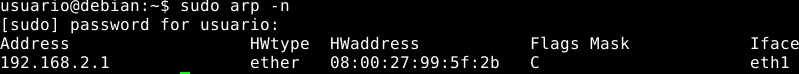
\includegraphics[width = \textwidth]{arptable_ex2}
        \caption{Tabla ARP de la máquina externa.}
      \end{figure}

    \subsection{Ataque 3}
      \par
      Ha cambiado la tabla del router, que ahora también reenvia los paquetes al
      atacante por lo cual en wireshark podemos ver los echo reply.

      \begin{figure}[H]
        \centering
        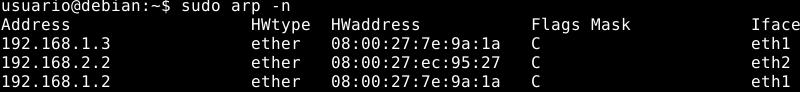
\includegraphics[width = \textwidth]{at_gw3}
        \caption{Tabla ARP del router.}
      \end{figure}

      \begin{figure}[H]
        \centering
        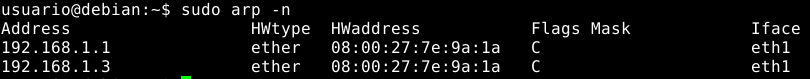
\includegraphics[width = \textwidth]{at_vic3}
        \caption{Tabla ARP de la víctima.}
      \end{figure}

      \begin{figure}[H]
        \centering
        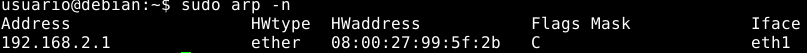
\includegraphics[width = \textwidth]{at_ex3}
        \caption{Tabla ARP de la máquina externa.}
      \end{figure}

  \section{Route cache poisoning con redirección ICMP}
    \par
    En las tablas de routa vemos que víctima envia a la red 2 mediante el
    atacante, en externo habla con víctima via el atacante. En wireshark podemos
    ver tanto los request como los reply.

    \begin{figure}[H]
      \centering
      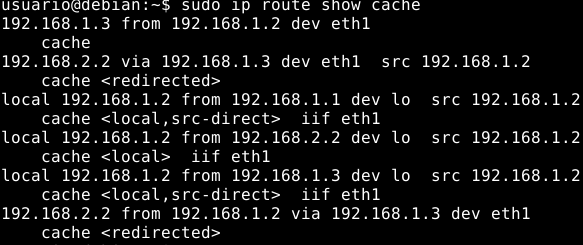
\includegraphics[width = \textwidth]{route_v}
      \caption{Route cache de la víctima.}
    \end{figure}

    \begin{figure}[H]
      \centering
      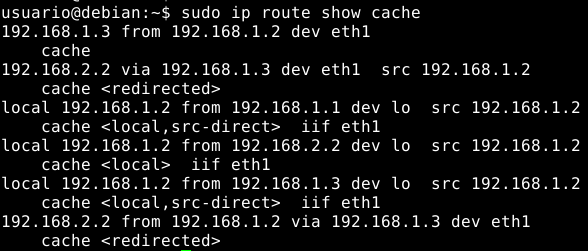
\includegraphics[width = \textwidth]{route_ex}
      \caption{Route cache de la máquina externa.}
    \end{figure}

  \section{ICMP/Ping flooding}
    \par
    El atacante esta enviado request continuamente a la víctima, para que esta
    no pueda continuar atendiendo peticiones (ocupando su ancho de banda).

  \section{Smurf Attack}
    \par
    Ahora esta realizando un broadcast en la red y todas las máquinas le están
    contestando por lo que esta boqueando la red 1 completa y no solo la máquina
    víctima.

  \section{TCP SYN flooding}
    \par
    Este ataque consiste en el envio masivo de paquetes TCP SYN a la víctima con
    el fin de que la generacion de respuestas por parte de esta la deje fuera de
    servicio.

    \subsection{Ataque 1}
      \par
      La máquina víctima sigue funcionando y su cpu no parece sufrir
      consecuencias, esto se debe a que al no recibir confirmación de su
      respuesta elimina los paquetes de la cola.

    \subsection{Ataque 2}
      \par
      A pesar de que recibe mayor número de paquetes tampoco se queda colgada,
      similar a lo que pasaba en el ataque anterior la máquina elimina las
      entradas que no reciben confirmación.
    \subsection{Ataque 3}
      \par
      Este ataque no tiene ningún impacto en la víctima, las ip origen son
      aleatorias y por tanto la máquina víctima no puede contestar por lo que
      ignora dichos paquetes.
    \subsection{Ataque 4}
      \par
      A diferencia de los otros ataques este "cuelga" a la víctima en el estado
      ACK wait, esto hace que las conexiones no se cierren y por tanto la cpu
      se inunde, este ataque si consigue inutilizar la máquina.

  \section{UDP flooding}
    \par
    No pudimos realizar este ataque porque la máquina atacante se colgaba al
    iniciarlo, pero su funcionamiento es idéntico al de TCP flooding solo
    cambiando los puertos a los que ataca.
\end{document}
